\section{Automated Testing-as-a-Service (TaaS)}


\section{Layered Symbolic Execution}

\subsection{Scaling on Commodity Shared-Nothing Clusters}
\label{sec:scalability}

We evaluate \cnine\ using two metrics:
\begin{enumerate}
\item The time to reach a certain goal (e.g., an exhaustive path exploration, or a fixed coverage level)---we consider this an \emph{external} metric, which measures the performance of the testing platform in terms of its end results.
\item The useful work performed during exploration, measured as the number of useful (non-replay) instructions executed symbolically. This is an \emph{internal} metric that measures the efficiency of \cnine's internal operation. 
%Useful instructions also mean that the shared prefixes of any two paths in the program are considered only once, according by this metric. 
\end{enumerate}

% In other words, from a scalability perspective, useful CPU hours are the ones performed by a single-node symbolic execution engine, when no communication or synchronization overhead is involved. This includes instruction execution and constraint solving. In this case, ineffective CPU hours are the ones used for bookkeeping, including replay work, and also idle CPU time. 

%\item The \emph{capacity}---how many paths the symbolic engine can accomodate at once. The unit of measure is the amount of memory, out of the total available, used for accomodating execution paths. Ideally, this should be proportionally to the total available RAM in the cluster, but in practice the memory is used for other purposes, as well. For instance, due to the way the job model is designed, \cnine\ maintains inactive states on each worker, which do not count towards the aggregated state frontier. The inactive states are used to speed up the replay process, therefore it's a "trade CPU for memory" case. 

A cluster-based symbolic execution engine \emph{scales} with the number of workers if these two metrics improve proportionally with the number of workers in the cluster.

\paragraph{Time Scalability} We show that \cnine\ scales linearly by achieving the same testing goal proportionally faster as the number of workers increases. We consider two scenarios.

First, we measure how fast \cnine\ can exhaustively explore a fixed number of paths in the symbolic execution tree.  For this, we use a symbolic test case that generates all the possible paths involved in receiving and processing two symbolic messages in the memcached server (\S\ref{sec:effectiveness} gives more details about the setup). Fig.~\ref{fig:scalab-time-vs-workers} shows the time required to finish the test case with a variable number of workers: every doubling in the number of workers roughly halves the time to completion.  With 48 workers, the time to complete is about 10 minutes; for 1 worker,  exploration time exceeds our 10-hour limit on the experiment.  

%The results of the experiment show an important aspect: while the path explosion problem cannot simply be solved by thowing more hardware at it, the size of the problems for which symbolic execution can be useful today are within the range in which a parallel symbolic execution engine can make a significant difference.

\begin{figure}[h!]
  \centering
  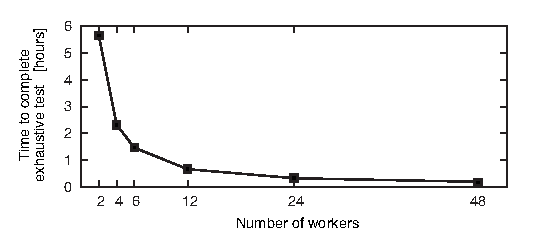
\epsfig{file=figures/evaluation/scalab-time-vs-workers-edited.eps, width=2.9in}
  \caption{\cnine\ scalability in terms of the time it takes to exhaustively complete a symbolic test case for memcached.}
  \label{fig:scalab-time-vs-workers}
\end{figure}

Second, we measure the time it takes \cnine\ to reach a fixed coverage level for the \codebit{printf} UNIX utility.  \codebit{printf} performs a lot of parsing of its input (format specifiers), which produces complex constraints when executed symbolically.   Fig.~\ref{fig:scalab-time-vs-workers-cov} shows that the time to achieve a coverage target decreases proportionally with the number of added workers.  The low 50\% coverage level can be easily achieved even with a sequential SEE (1-worker \cnine). However, higher coverage levels require more workers, if they are to be achieved in a reasonable amount of time; e.g., only a 48-worker \cnine is able to achieve  $90\%$ coverage.  The anomaly at 4 workers for 50\% coverage is due to high variance; when the number of workers is low, the average (5$\pm$4.7 minutes over 10 experiments) can be erratic due to the random choices in the random-path search strategy.

\begin{figure}[h!]
  \centering
  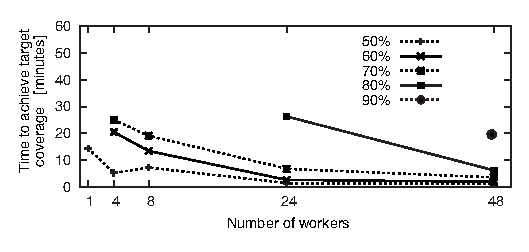
\epsfig{file=figures/evaluation/scalab-time-vs-workers-cov-printf-edited.eps, width=2.9in}
  \caption{\cnine\ scalability in terms of the time it takes to obtain a target coverage level when testing \codebit{printf}.}
  \label{fig:scalab-time-vs-workers-cov}
\end{figure}

\paragraph{Work Scalability} We now consider the same scalability experiments from the perspective of useful work done by \cnine: we measure both the total number of instructions (from the target program) executed during the exploration process, as well as normalize this value per worker. This measurement indicates whether the overheads associated with parallel symbolic execution impact the efficiency of exploration, or are negligible. Fig.~\ref{fig:scalab-memcached} shows the results for memcached, confirming that \cnine scales linearly in terms of useful work done (top graph).  The average useful work done by a worker (bottom graph) is relatively independent of the total number of workers in the cluster, so adding more workers improves proportionally \cnine's results.

\begin{figure}[t!]
  \centering
  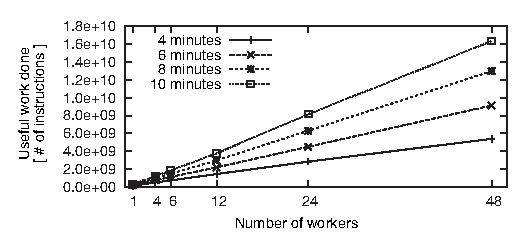
\epsfig{file=figures/evaluation/scalab-thr-cpu-vs-workers-memcached-edited.eps, width=2.9in} \\
  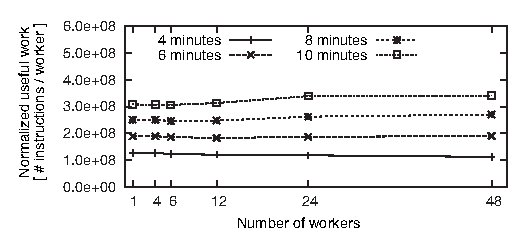
\epsfig{file=figures/evaluation/scalab-thr-cpu-perc-vs-workers-memcached-edited.eps, width=2.9in}
  \caption{\cnine\ scalability in terms of useful work done for four different running times when testing memcached.}
  \label{fig:scalab-memcached}
\end{figure}

% However, we noticed a different effect even on the \codebit{printf} utility (Fig.~\ref{fig:scalab}). Contrary to intuition, the total useful work effort scales super-linearly.  In other words, the average efficiency of a worker \emph{grows} with the number of total workers in the cluster.

% This is because parallel exploration favors a quicker exploration of the parts of the symbolic execution tree with low constraint solving overhead, and thus yields higher instruction throughput.  Even if each worker node runs the same strategy, at a global level the "distributed" strategy of selecting the nodes in the global frontier depends on how the frontier is partitioned among workers.  Many small partitions give more chances to each segment of the frontier to be selected, and thus reduce the probability of bottlenecking in parts of the tree with high instruction execution times caused by complex constraint solving.

% The effect is barely noticeable in the case of memcached because in that case, the exploration is exhaustive and the same instructions are eventually executed regardless of the selection strategy.

In Fig.~\ref{fig:scalab} we show the results for \codebit{printf} and \codebit{test}, UNIX utilities that are an order of magnitude smaller than memcached. We find that the useful work done scales in a similar way to memcached, even though the three programs are quite different from each other (e.g., \codebit{printf} does mostly parsing and formatting, while memcached does mostly data structure manipulations and network I/O).


\begin{figure}[h!]
  \centering
  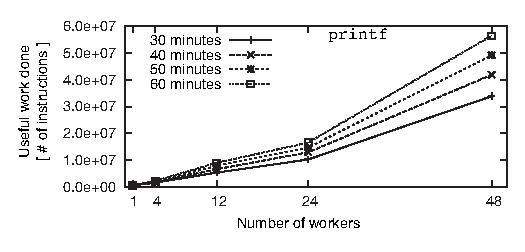
\epsfig{file=figures/evaluation/scalab-thr-cpu-vs-workers-edited.eps, width=2.9in} \\
  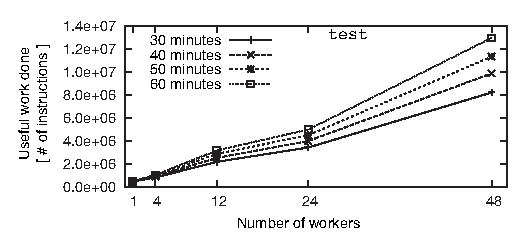
\epsfig{file=figures/evaluation/scalab-thr-cpu-vs-workers-test-edited.eps, width=2.9in}
  \caption{\cnine's useful work on \codebit{printf} (top) and \codebit{test} (bottom) increases roughly linearly in the size of the cluster.}  
  \label{fig:scalab}
\end{figure}

In conclusion, \cnine scales linearly with the number of workers, both in terms of the time to complete a symbolic testing task and in terms of reaching a target coverage level.  % As far as the performed work is concerned, we observe that worker efficiency increases as the total number of workers in the system increases.

\subsection{Utility of Load Balancing}
\label{sec:profiling}
 
In this section we explore the utility of dynamic load balancing.  Consider the example of exhaustively exploring paths with two symbolic packets in memcached, using 48 workers, but this time from a load balancing perspective. Fig.~\ref{fig:scalab-load-balancing} shows that load balancing events occur frequently, with \linebreak 3--6\% of all states in the system being transferred between workers in almost every 10-second time interval.

\begin{figure}[h!]
  \centering
  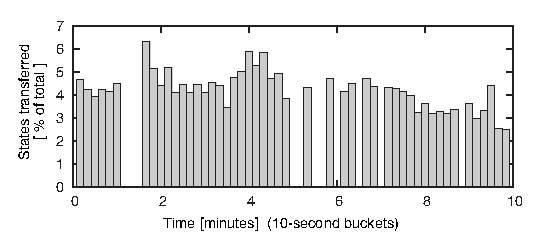
\epsfig{file=figures/evaluation/scalab-load-balancing-edited.eps, width=3in}
  \caption{The fraction of total states (candidate nodes) transferred between workers during symbolic execution.}
  \label{fig:scalab-load-balancing}
\end{figure} 

To illustrate the benefits of load balancing, we disable it at various moments in time and then analyze the evolution of total useful work done. Fig.~\ref{fig:scalab-static-balancing} shows that the elimination of load balancing at any moment during the execution significantly affects the subsequent performance of exploration due to the ensuing imbalance.  This demonstrates the necessity of taking a dynamic approach to parallel symbolic execution, instead of doing mere static partitioning of the execution tree.

%Scaling symbolic execution is a hard problem. A naive approach to parallelization, e.g. static splitting of the search space, does not give good performance in general. Figure~\ref{fig:scalab-static-split} shows side by side \cnine with N nodes and the Klee symbolic execution engine with a statically split search space.

%The load balancer is indeed a necessary component. Figure~\ref{fig:scalab-load-balancing} shows the distribution of the load balancing decisions during \cnine\ execution (\stefan{Experiment done with 24 workers, on memcached with 2 sequential symbolic binary commands.}).

\begin{figure}[h!]
  \centering
  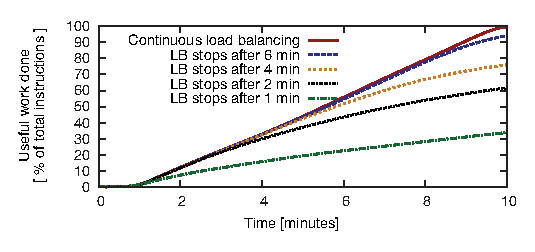
\epsfig{file=figures/evaluation/scalab-static-balancing-edited.eps, width=3in}
  \caption{Instruction throughput of \cnine\ with load balancing disabled at various points during the exhaustive test.}
  \label{fig:scalab-static-balancing}
  \vspace{-0.5cm}
\end{figure}

\subsubsection{Case Study \#1: UNIX Utilities}
\label{sec:coreutils}

\topic{\klee is an excellent tool for testing command-line programs, in particular \unix utilities.}  It does not tackle more complex systems, like the ones in Table~\ref{table:tested}, mainly due to path explosion (since \klee is a single-node engine) and insufficient environment support.  We cannot compare \cnine to \klee on parallel and distributed systems, but we can compare on the Coreutils suite of \unix utilities~\cite{coreutils}.

We run \klee on each of the 96 utilities for 10 minutes, and then  run a 12-worker \cnine on each utility for 10 minutes. Fig.~\ref{fig:coreutils-cov} reports the average coverage increase obtained with \cnine over 7 trials, using \klee's 7-trial average results as a baseline; the experiment totals $2 \times 7 \times 96 \times 10 = 13,440$ minutes $>$ 9 days.  The increase in coverage is measured as {\em additional} lines of code covered, expressed as a percentage of program size (i.e., we do not report it as a percentage of the baseline, which would be a higher number).

\topic{\cnine covers up to an additional $40\%$ of the target programs, with an average of $13\%$ additional code covered across all Coreutils.}  In general, improving coverage becomes exponentially harder as the base coverage increases, and this effect is visible in the results: a $12\times$ increase in hardware resources does not bring about a $12\times$ increase in coverage.  Our results show that \cnine allows ``throwing hardware'' at the automated testing problem, picking up where \klee left off.  In three cases, \cnine achieved $100\%$ coverage in 10 minutes on real-world code.  This experiment does not aim to show that \cnine is a ``better'' symbolic execution engine than \klee---after all, \cnine is based on \klee---but rather that \cnine-style parallelization can make existing symbolic execution engines more powerful.

The way we compute coverage is different from~\cite{klee}---whereas \klee was conceived as an automated {\em test generator}, \cnine is meant to {\em directly test} software. Thus, we measure the number of lines of code tested by \cnine, whereas \cite{klee} reports numbers obtained by running the concrete test cases generated by \klee.  Our method yields more-conservative numbers because a test generated by \klee at the end of an incomplete path (e.g., that terminated due to an environment failure) may execute further than the termination point when run concretely.

\begin{figure}[h!]
  \centering
  \label{fig:coreutils-final-cov}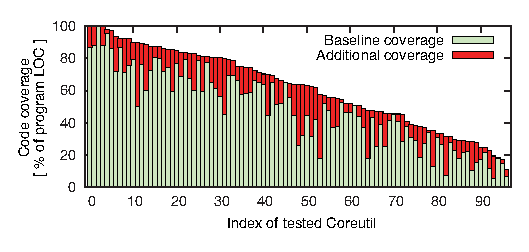
\epsfig{file=figures/evaluation/coreutils-cov-edited.eps, width=3.2in} \\
  \label{fig:coreutils-delta-cov}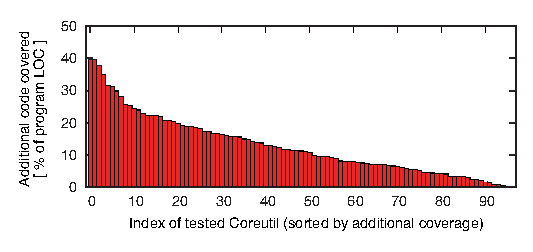
\epsfig{file=figures/evaluation/coreutils-delta-cov-edited.eps, width=3.2in}
  \caption{\cnine coverage improvements on the 96 Coreutils (1-worker \cnine vs. 12-worker \cnine).}
  \label{fig:coreutils-cov}
\end{figure}


%%% Local Variables: 
%%% mode: latex
%%% eval: (visual-line-mode)
%%% fill-column: 1000000
%%% TeX-master: "main"
%%% End:
